\begin{figure}
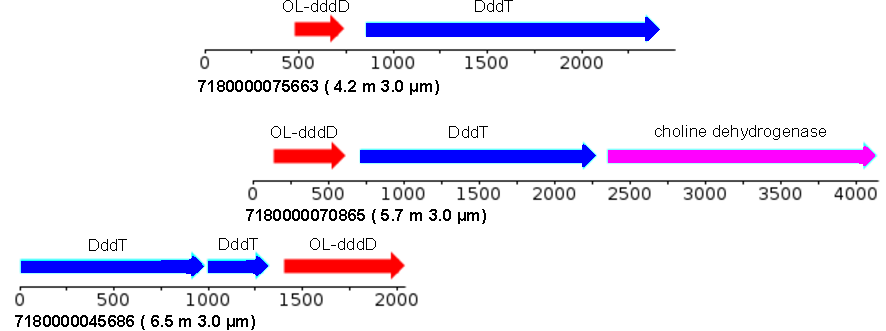
\includegraphics[width=\textwidth]{orglake_figures/OLdddD_scaffolds.pdf}
\caption[Maps of OL-dddD-containing scaffolds]{Genomic maps of Organic Lake scaffolds containing the OL-dddD homologue. DddT and choline dehydrogenase had best \ac{BLAST} matches to \emph{Halomonas} sp. HTNK1 (\emph{Gammaproteobacteria}) and \emph{Hoeflea phototrophica} DFL-43 (\emph{Alphaproteobacteria}), respectively. The numbers represent base pairs. The sample depth and filter from which the scaffold was assembled is shown in parentheses beside the scaffold ID.}
\label{fig:OLdddD_scaffolds}

\end{figure}
